<<<<<<< HEAD
\newpage
\section{Auswertung}
\subsection{Wertetabelle}
\begin{table}[H]
    \centering
    \begin{tabular}{c | c c c c c}
        \toprule
        & Feder 1 & Feder 2 & Feder 3 & Feder 4 & Feder 5 \\ & (Basisfeder)\\
        \midrule
        $m\;/\;$g & 1.3456 & 1.311 & 1.3812 & 1.4574 & 1.2342 \\
        \midrule
        $D_a\;/\;$mm & 3.68 & 3.57 & 3.82 & 3.69 & 3.69 \\
          & 3.67 & 3.57 & 3.81 & 3.68 & 3.69 \\
          & 3.69 & 3.57 & 3.82 & 3.68 & 3.68 \\
          & 3.68 & 3.57 & 3.82 & 3.68 & 3.68 \\
          & 3.69 & 3.57 & 3.82 & 3.76 & 3.68 \\
          & 3.68 &         &         &         &         \\
        \midrule
        $\bar{D_a}\;/\;$mm & 3.68* & 3.57 & 3.818 & 3.69 & 3.684\\
        $D_{a_S}\;/\;$mm& 0.007 & 0 & 0.004 & 0.03 & 0.005\\
        \midrule
        $L_a\;/\;$mm & 58.76 & 59.02 & 58.1 & 62.87 & 54.45 \\
          & 58.89 & 59.11 & 58.41 & 62.94 & 54.53 \\
          & 58.79 & 58.99 & 58.32 & 63.03 & 54.58 \\
          & 58.88 & 59.13 & 58.38 & 63.01 & 54.69 \\
          & 58.61 & 58.99 & 58.61 & 62.92 & 54.54 \\
          & 58.76 &         &         &         &         \\
        \midrule
        $\bar{L_a}\;/\;$mm & 58.78 & 59.048 & 58.364 & 62.95 & 54.55\\
        $L_{a_S}\;/\;$mm & 0.09 & 0.06 & 0.16 & 0.059 & 0.078\\
        $n$ & & & & & \\
        \midrule
        $F1\;/\;$N bei $L1=105\;$mm & 4.8 & 5.21 & 4.46 & 4.26 & 5.5\\
                         & 4.86 & 5.28 & 4.48 & 4.25 & 5.5\\
                         & 4.83 & 5.29 & 4.5 & 4.3 & 5.48\\
                         & 4.83 & 5.28 & 4.49 & 4.28 & 5.47\\
                         & 4.85 & 5.29 & 4.52 & 4.23 & 5.49\\
        \midrule
        $F2\;/\;$N bei $L2=142\;$mm & 7.97 & 8.7 & 7.33 & 7.2 & 8.93\\
                         & 8.02 & 8.75 & 7.33 & 7.17 & 8.92\\
                         & 7.96 & 8.73 & 7.35 & 7.22 & 8.93\\
                         & 8.0 & 8.75 & 7.35 & 7.2 & 8.9\\
                         & 8.04 & 8.77 & 7.4 & 7.14 & 8.93\\
        \midrule
        $\bar{F1}\;/\;$N & 4.83 & 5.27 & 4.49 & 4.264 & 5.49\\
        $\bar{F2}\;/\;$N & 7.99 & 8.74 & 7.35 & 7.19 & 8.92\\
        \midrule
        $R$ & 0.086 & 0.094 & 0.077 & 0.079 & 0.093\\
        \midrule
        $F_0\;/\;$N & 0.88 & 0.96 & 0.88 & 0.94 & 0.81\\ 
        \bottomrule
    \end{tabular}
    \caption{$m$ Federmasse,
             $D_a$ Federaußendruchmesser, 
             $\bar{D_a}$ Mittelwert des Federaußendruchmesser, 
             $D_{a_S}$ Standartabweichung des Federaußendruchmesser,
             $L_0$ Federlänge,
             $\bar{L}$ Mittelwert der Federlänge,
             $L_{0_S}$ Standartabweichung der Federlänge,
             $n$ Windungszahl,
             $F1$,$F2$ Federkräfte,
             $\bar{F1}$,$\bar{F2}$ Mittelwert der Federkräfte,
             $R$ Federkonstante,
             $F_0$ Innere Vorspannkraft\\
             * Wird im folgenden als Basiswert verwendet
    }
    \label{tab:Wertetabelle}
\end{table}


\subsection{Variable Federdicke}
\begin{figure}[H]
    \center
    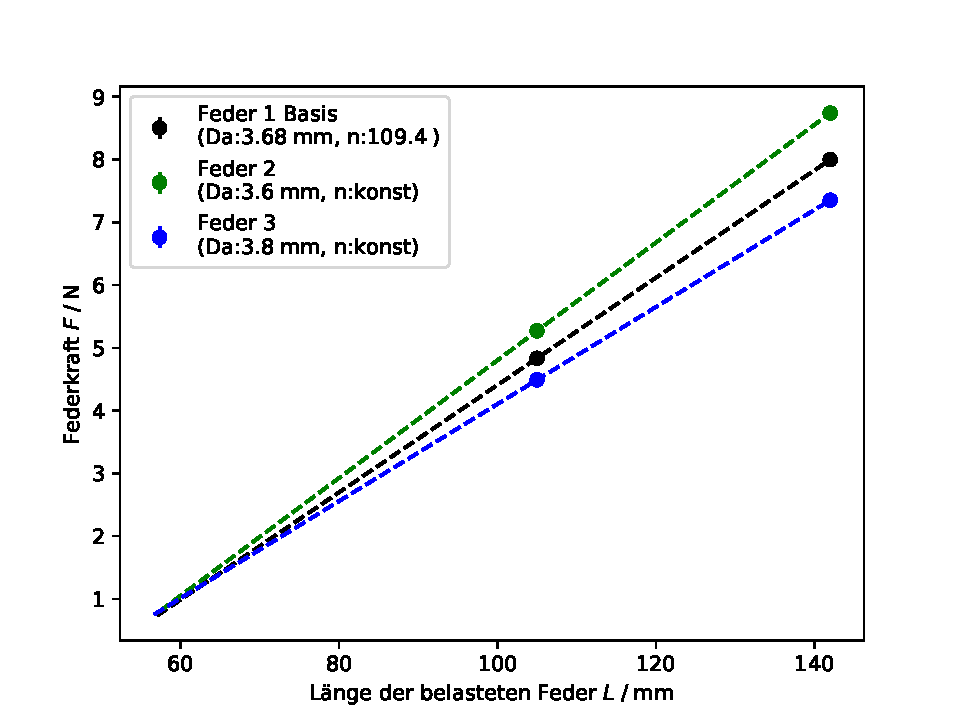
\includegraphics[width=0.9\textwidth]{build/D_kraftweg_dia.pdf}
    \caption{Feder 1,2,3 mit unterschiedlichen Federdurchmessern $D$ bei konstanter Basis Federwindungszahl $n$.
    Aufgetragen in einem Kraft-Weg-Diagramm. Gemessen wurden dabei
    die für L1 und L2 resultierenden Federkräfte F1 und F2.}
    \label{tab:LF_D}
\end{figure}
\subsection{Lineare Ausgleichsgerade}
\label{sec:fit}
Für die jeweiligen Ausgleichsgeraden aus \ref{tab:LF_D} wird ein Polyfit \cite{numpy_polyfit}
ersten Grades durchgeführt und daraus die Steigung, also die Federkonstante $R$ so wie eine Verschiebung
in der vertikalen $v$ ermittelt.\\
Aus \ref{eqn:federrate} mit
\begin{equation}
  F=R \cdot s + v ,
\end{equation}
folgen somit die in \ref{tab:Wertetabelle} aufgeführten Federkonstanten.
\begin{align*}
  R1= 0.086\;\si{\N\per\mm}, &&  v1= -4.14\;\si{\N},\\
  R2= 0.094\;\si{\N\per\mm}, &&  v2= -4.58\;\si{\N},\\
  R3= 0.077\;\si{\N\per\mm}, &&  v3= -3.63\;\si{\N}.\\
\end{align*}

\subsection{Innere Vorspannkraft ermitteln}
\label{sec:vorspannkraft}
Um nun aus den Verschiebungswerten $v$ auf die innere Vorspannkraft $F_0$ verschiebe
man die Gerade so, dass nun der Federweg $\Delta L$ betrachtet wird.
Die Kraft $F_0$, die zuvor bei der Federlänge $L_0$ lag, liegt nun bei $\Delta L=0$
und beschreibt die zugehörige Vorspannkraft $F_0$.
\begin{figure}[H]
  \center
  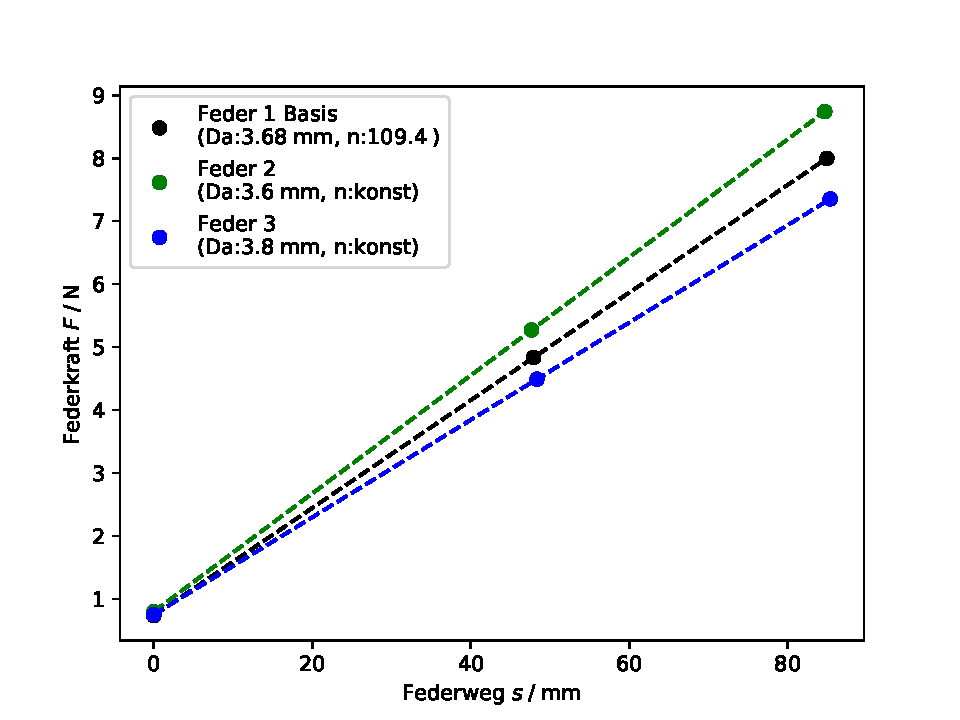
\includegraphics[width=0.9\textwidth]{build/f0_123_dia.pdf}
  \caption
  {
    Federkraft $F$ betrachtet für $\Delta L$,y-Achsenabschnittet bildet dabei die innere Vorspannkraft $F_0$.
    So folgt aus einer Geradengleichung mit $y_0=R\cdot(L-L_0)+b$ dass $y_{\Delta L}=y_0+R \cdot L_0=R \cdot L+b$
    wobei für $L=0$ folglich gilt $y_{\Delta L}(L=0)=b:=F_0$.
  }
\end{figure}
Somit ergeben sich für die jeweilligen inneren Vorspannkräfte $F_0$
\begin{align*}
  F1_0=  0.88 \;\si{\N},\\
  F2_0=  0.96 \;\si{\N},\\
  F3_0=  0.88 \;\si{\N}.\\
\end{align*}



\begin{figure}[H]
  \center
  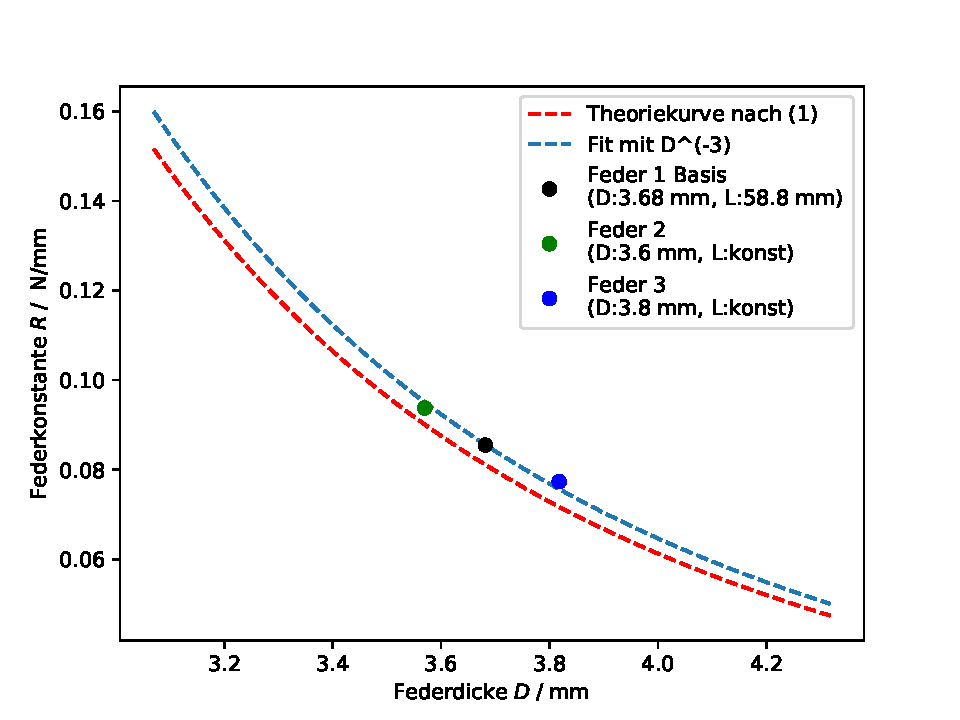
\includegraphics[width=0.9\textwidth]{build/dicke_konstante_dia.pdf}
  \caption{Die Federdicke $D_a$ gegen die Federkonstante $R$ aufgetragen.}
\end{figure}

\subsubsection{Ausgleichsgerade}

Es folgt aus \ref{eqn:federrate}
\begin{align*}
  R=\frac{G\;d^4}{8\;n}\cdot \frac{1}{D^3}, \\\\  
  \text{mit }k_D =\frac{G\;d^4}{8\;n},
\end{align*}
Es folgt die Funktion
\begin{equation*}
  R(D)=k_D \cdot \frac{1}{D^3},
\end{equation*}
mit dem Parameter
\begin{equation*}
  k_D=(4.28 \pm 0.012) \;\si{\N\meter\squared}
\end{equation*}


\subsection{Variable Federwindungszahl}
\begin{figure}[H]
    \center
    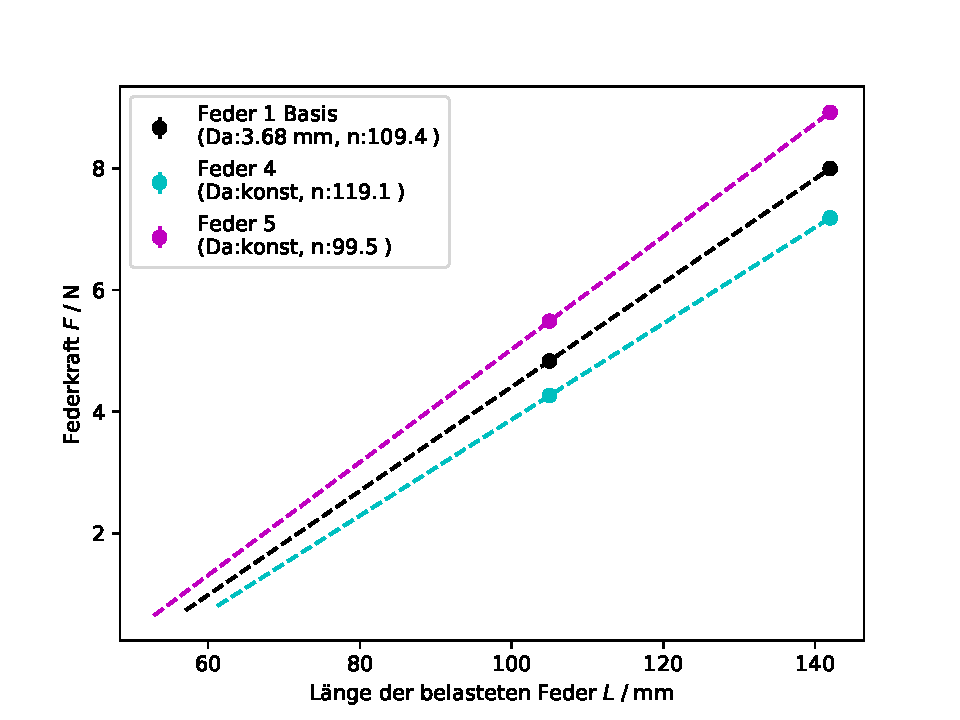
\includegraphics[width=0.9\textwidth]{build/n_kraftweg_dia.pdf}
    \caption{Feder 1,4,5 mit unterschiedlichen Windungszahlen $n$ bei konstanter Basis Federdicke $D_a$.
    Aufgetragen in einem Kraft-Weg-Diagramm. Gemessen wurden dabei die für L1
    und L2 resultierenden Federkräfte F1 und F2}
\end{figure}
Analog wie in Abschnitt \ref{sec:fit} folgt für die Federkonstante $R$
und den Verschiebungswert $v$ aus dem mit der Methodik aus \ref{sec:vorspannkraft}
die innere Vorspannkraft $F_0$ ermittelt wird
\begin{align*}
  R1= 0.086\;\si{\N\per\mm}, &&  v1= -4.14\;\si{\N}, && F1_0=0.88\;\si{\N}\\
  R4= 0.079\;\si{\N\per\mm}, &&  v4= -4.03\;\si{\N}, && F4_0=0.94\;\si{\N}\\
  R5= 0.092\;\si{\N\per\mm}, &&  v5= -4.26\;\si{\N}. && F5_0=0.81\;\si{\N}\\
\end{align*}

\begin{figure}[H]
  \center
  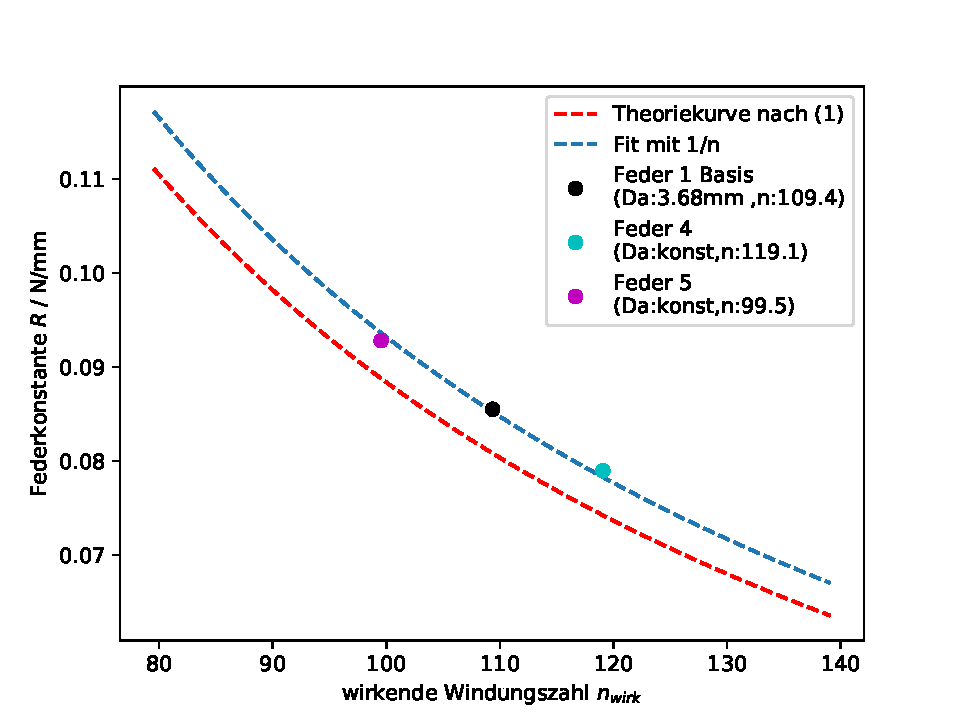
\includegraphics[width=0.9\textwidth]{build/n_konstante_dia.pdf}
  \caption{Einfluss der Windungszahl $n$ auf die Federkonstante $R$}
\end{figure}

\subsubsection{Ausgleichsgerade}

Es folgt aus \ref{eqn:federrate}
\begin{align*}
  R=\frac{G\;d^4}{8\;D^3}\cdot \frac{1}{n} \\\\  
  \text{mit } k_n=\frac{G\;d^4}{8\;D^3}
\end{align*}
Es folgt die Funktion
\begin{equation*}
  R(n)=k_n \cdot \frac{1}{n}
\end{equation*}
mit dem Parameter
\begin{equation*}
  k_n=(11.69 \pm 0.06) \;\si{\N\meter\squared}
\end{equation*}


\subsection{Betrachtung der Masse}
\begin{figure}[H]
  \center
  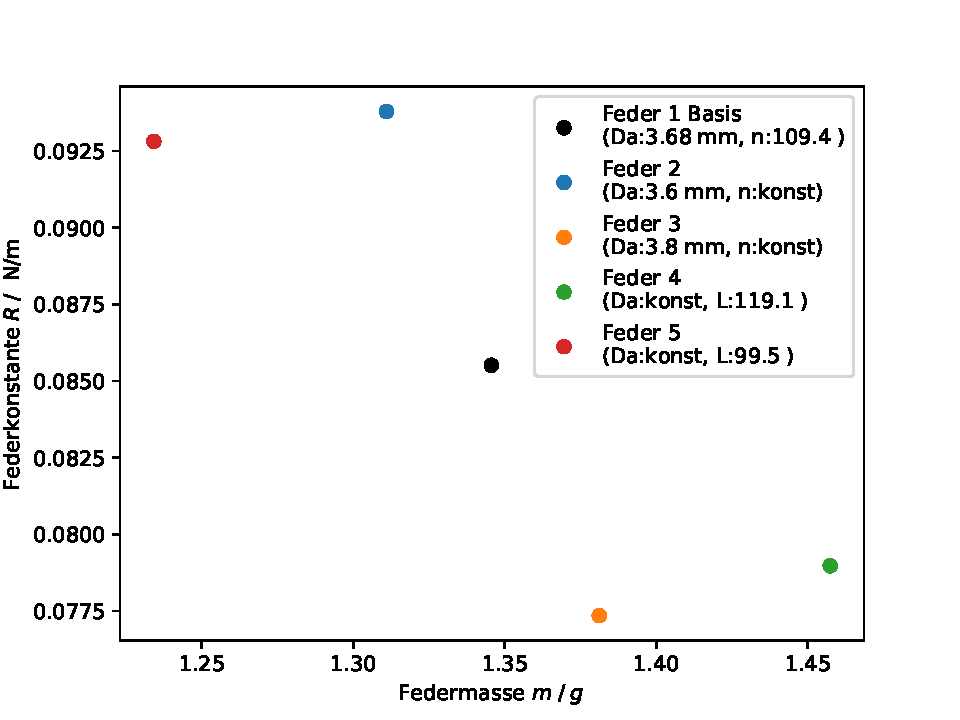
\includegraphics[width=0.9\textwidth]{build/masse_konstante_dia.pdf}
  \caption{Massenresulate aus der Variation der Federdicke $D_a$
          und der Windungszahl $n$ der Federkonstanten $R$ gegenübergestellt. }
\end{figure}



\label{sec:Auswertung}
||||||| merged common ancestors
=======
\newpage
\section{Auswertung}
\label{sec:Auswertung}
>>>>>>> 4725ae2bea169a0e96b27f3c21c1fb3c50c57da5
